%%%%%%%%%%%%%%%%%%%%%%%%%%%%%%%%%%%%%%%%%%%%%%%%%%%%%%%%%%%%%%%%%%%%%%%%%%% 
% Nombre del trabajo, 
% t�tulo,
% autores
% fechas, 
% comentarios, etc.
%%%%%%%%%%%%%%%%%%%%%%%%%%%%%%%%%%%%%%%%%%%%%%%%%%%%%%%%%%%%%%%%%%%%%%%%%%% 
%\input miscomandos.tex % Comandos definidos por el autor

%\documentclass[a4paper,12pt]{book} 

%% Incluir los paquetes necesarios 
%\usepackage[latin1]{inputenc} % Caracteres con acentos. 
%\usepackage[spanish]{babel}
%\usepackage{latexsym} % Simbolos 
%\usepackage[pdftex=true,colorlinks=true,plainpages=false]{hyperref} % Soporte hipertexto
%\usepackage[pdftex]{graphicx} %Inclusión de gr�ficos PDFLaTeX
%\DeclareGraphicsExtensions{.png,.pdf,.jpg}
%\renewcommand{\baselinestretch}{1.5} %espacio entre lineas
%\sloppy % suaviza las reglas de ruptura de l�neas de LaTeX

% T�tulo, autor, fecha. 
\title{capitulo1} 
\author{Angel baltar Diaz}
\date{\Large Enero, 2010} 

%\begin{document} % Inicio del documento
%capitulo 1 introduccion
\chapter {El juego}
\label{capitulo1}

En este capítulo presentaremos el juego, su temática, estilo y cual es la concepción general del título, que es lo que hace hasta el momento y cuales son en general las líneas de trabajo que están planteadas.

\section{Temática del juego}

Este juego se basa en la típica temática de guerra entre naves espaciales, es un juego estilo R-type en el que el jugador maneja una única nave y debe destruir ejércitos enteros de naves enemigas, dentro de este estilo de juego la temática en si está abierta, no hay una historia concreta en la que el juego se base por el momento.

Se ha planteado desde un principio una temática basada en el universo star Trek en el que el protagonista es un klingon que toma una nave por su cuenta y se lanza a conquistar territorios enemigos, sin embargo como ya decía la temática esta completamente abierta mientras se mantenga el estilo de juego. Si en algun momento se quiere prescindir de la temática basada en star trek por temas de licencias o por cualquier otro motivo, no habría problema en hacerlo, además tecnicamente es simplemente cambiar imágenes de naves, fondos de los escenarios, logos etc. 

\begin{figure}[t]
\centering
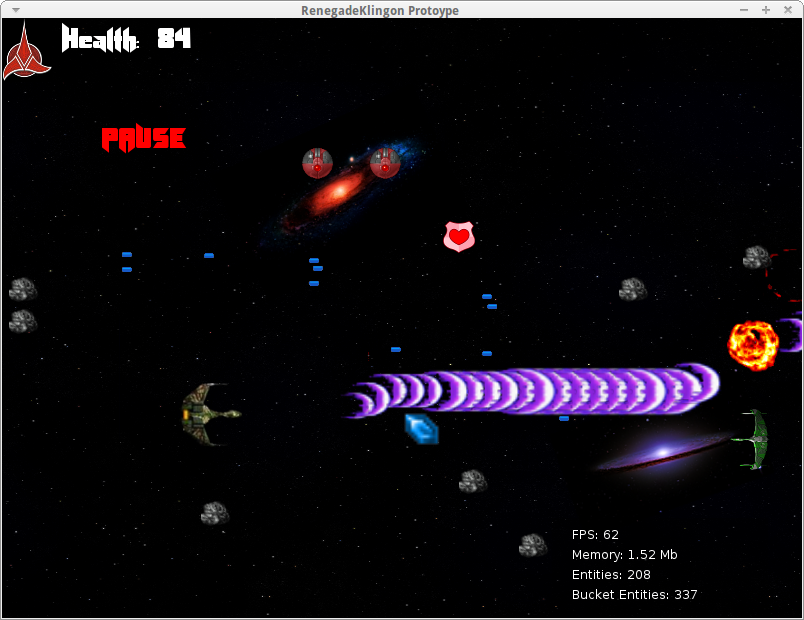
\includegraphics[width=\linewidth]{includes/images/Screen_Shoot1.png}
\caption{Captura de pantalla del juego}
\label{fig:RenegadeKlingonScreenShoot}
\end{figure}


%section objetivos
\section{Objetivos}

Este juego surje como un simple hobby, he estado dedicando tiempo libre a su construcción, en general las partes de programación no me plantean excesivos problemas, sin embargo tengo lagunas muy importantes en el apartado gráfico porque no sé lo suficiente de diseño gráfico.
Tal como he planteado el juego los objetivos que tengo para el son los siguientes:

\begin{itemize}
\item Juego en 2d estilo \textbf{R-type}[\ref{glosario}].
\item Niveles diseñables y extensibles sin necesidad de programar (basados en generación mediante Tiled).
\item Armas intercambiables que se puedan ir consiguiendo durante el juego.
\item Sistema de juego basado en nivel de salud combinable con número de vidas.
\item Soporte como aplicación de escritorio para Mac, Windows y linux
\item Soporte para dispositivos móviles
\item Soporte para jugar a través de Web
\end{itemize}

Algunos de estos objetivos están actualmente cumplidos, otros son en principio tecnicamente viables y de otros simplemente aun no he mirado como pueden hacerse, en otros capítulos entraremos más en detalles técnicos sobre todas estas cuestiones.

%\end{document} % Fin del documento
